\documentclass[12pt]{article}
\usepackage[T1]{fontenc}
\usepackage{calc}
\usepackage{setspace}
\usepackage{multicol}
\usepackage{fancyheadings}

\usepackage{natbib}
 
\usepackage{graphicx}
\usepackage{color}
\usepackage{rotating}
\usepackage{verbatim}
\usepackage{array}
\usepackage{multirow}

\setlength{\voffset}{-0.25in}
\setlength{\topmargin}{0pt}
\setlength{\hoffset}{-0.2in}
\setlength{\oddsidemargin}{0pt}
\setlength{\headheight}{0pt}
\setlength{\headsep}{.4in}
\setlength{\marginparsep}{0pt}
\setlength{\marginparwidth}{0pt}
\setlength{\marginparpush}{0pt}
\setlength{\footskip}{.1in}
\setlength{\textwidth}{6.9in}
\setlength{\textheight}{9.25in}
\setlength{\parskip}{0pc}

\renewcommand{\baselinestretch}{0.85}

\newcommand{\bi}{\begin{itemize}}
\newcommand{\ei}{\end{itemize}}
\newcommand{\be}{\begin{enumerate}}
\newcommand{\ee}{\end{enumerate}}
\newcommand{\bd}{\begin{description}}
\newcommand{\ed}{\end{description}}
\newcommand{\prbf}[1]{\textbf{#1}}
\newcommand{\prit}[1]{\textit{#1}}
\newcommand{\beq}{\begin{equation}}
\newcommand{\eeq}{\end{equation}}
\newcommand{\bdm}{\begin{displaymath}}
\newcommand{\edm}{\end{displaymath}}
\newcommand{\script}[1]{\begin{cal}#1\end{cal}}
\newcommand{\citee}[1]{\citeauthor{#1} (\citeyear{#1})}
\newcommand{\h}[1]{\hat{#1}}
\newcommand{\ds}{\displaystyle}
\newcommand{\normal}{\mathcal{N}}
\newcommand{\app}
{
\appendix
}

%\newcommand{\appsection}[1]
%{
%\let\oldthesection\thesection
%\renewcommand{\thesection}{Appendix \oldthesection}
%\section{#1}\let\thesection\oldthesection
%\renewcommand{\theequation}{\thesection\arabic{equation}}
%\setcounter{equation}{0}
%}

\newcommand{\appsection}[1]
{
\section{#1}
\renewcommand{\theequation}{\thesection\arabic{equation}}
\setcounter{equation}{0}
}

\renewcommand{\section}[1]{\addtocounter{section}{1} \begin{center}\textbf{\thesection~ #1}\end{center}}
\renewcommand{\subsection}[1]{\addtocounter{subsection}{1}\begin{center}\textbf{\thesubsection~ #1}\end{center}}

\pagestyle{empty}
\renewcommand{\thetable}{\Roman{table}}

\begin{document}

\noindent ``Improving the public's understanding of the central bank's objectives and policy strategies reduces economic and financial uncertainty and thereby allows business and households to make more informed decisions.''
$\sim$ Ben S. Bernanke, Speech to the Cato Institute 25th Annual Monetary Conference, November 17, 2007.

\section{Introduction}
Bernanke demonstrates in this quote that the Federal Reserve recognizes the value in keeping the public informed about the conduct of monetary policy.  Even so, the Federal Reserve has a dual mandate to promote both employment and inflation stability, it does not explicitly communicate relative importance for each of these goals, and it does not communicate an explicit long-run target for inflation as central banks from some other countries do.  One might argue the reason for being vague is to give monetary policy flexibility to address new short-run economic challenges while maintaining credibility to keep inflation at moderate levels in the long run.  However, the lack of complete communication concerning the conduct of monetary policy may create some uncertainty among market participants concerning short-run and long-run monetary policy actions.  The purpose of this paper is to measure the degree of monetary policy uncertainty in the U.S. economy over the last several decades, and examine the effect uncertainty has on levels of output growth, unemployment, inflation, and the volatility of these variables.

Many authors have found monetary policy transparency and credibility important are for macroeconomic stability.  For example, \citee{cecchetti_krause2002} find evidence for this from 60 central banks around the world.  \citee{cecchetti2006} find for 20 countries around the world that 80\% of the reduction in macroeconomic volatility since the early 1980s can be attributed to better monetary policy, and that credibility and transparency plays an important role.  \citee{bernanke1997} suggests that the decrease in macroeconomic volatility since the early 1980s in the United States was due in large part to an established, and therefore well understood, monetary policy that put its greatest emphasis on inflation targets.  \citee{cecchetti_ehrmann2002} similarly find evidence for countries across the world that central banks that have shifted focus to inflation stability, either explicitly or implicitly, have sucessfully limited both inflation and output volatility since the early 1980s.

All these papers suggest that monetary policy that is well understood by the public leads greater macroeconomic stability, and many attribute the slow down of macroeconomic volatility around the world since the early 1980s to precisely this.  A related literature examines the effect macroeconomic volatility has on levels of inflation and output growth, where volatility is used as a measure for economic uncertainty.  Examples from this literature include \citee{grier_perry2000}, \citee{fountas2001}, \citee{fountas2002}, \citee{grier2004}, \citee{fountas2006}, and \citee{fountas2007}.  All these papers use autoregressive heteroskedastic models, with varying complications, to establish measures of economic uncertainty.  While results sometimes depend on the specification of the model, most of the papers agree that higher inflation uncertainty has a negative impact on economic growth.  In a sense, the implication for monetary policy may agree with \citee{bernanke1997} in that successful inflation targeting can lead to better macroeconomic outcomes.

The above papers are limited in that they do not focus specifically on uncertainty concerning monetary policy, and they cannot separate heteroskedasticity and uncertainty, so as to determine the impact uncertainty has volatility.  The present paper takes a step in each of these directions.  Motivated by the literature on transparency and inflation targeting which suggests well-understood policy leads to desirable outcomes, the present work measures monetary policy uncertainty in the U.S. by measuring market participants perceptions of monetary policy.  Specifically, we suppose agents estimate a Taylor-like regression rule where the federal funds rate responds to expectations of future inflation, output growth, and unemployment.  Since the Fed does not explicitly communicate the relative importance of inflation and employment stability, the target inflation rate, or how responsive the federal funds rate is to fluctuations in these variables, we argue monetary policy is transparent when its actions are predictable, based on estimates of the linear regression monetary policy rule using data available to agents at the time.  

We re-estimate the Taylor-like regression rule for each period in our sample, using only the data prior to this period which would realistically be available to market participants at the time.  Specifically, we use a constant-gain least squares learning algorithm in the style of \citee{evanshonka2001} which supposes agents give relatively more weight to more recent observations.  We use the root mean squared error from this regression as our measure of monetary policy uncertainty and report the evolution of agents' perceptions and agents' levels of uncertainty over the sample period.  We then estimate the impact uncertainty has on levels of output growth, unemployment and inflation and the volatility of these variables.  We fail to find evidence that uncertainty affects the levels of these variables, but in many specifications we consider, we find statistically significant evidence that greater monetary policy uncertainty leads to greater volatility of output growth, unemployment, and inflation.

\section{Estimating Monetary Policy}
\subsection{Data}
To generate rolling estimates of the Taylor rule and compute estimates for monetary policy uncertainty, we use quarterly data from 1978:Q4 through 2011:Q3 on the federal funds rate and expected future output growth, inflation, and unemployment using the median forecast from the Survey of Professional Forecasters.  To estimate the impact that monetary policy uncertainty has on macroeconomic outcomes, we use quarterly data from the same time period on output growth, inflation, unemployment, and the federal funds rate.  Output growth is measured using the annualized quarterly percentage growth rate in real GDP, and inflation is measured using the annualized quarterly percentage growth rate in the GDP deflator.  

\subsection{Least Squares Learning}
Agents learn how the Federal Reserve conducts monetary policy by estimating the following policy rule similar to Taylor (1993),
\beq \label{eq:taylor} r_t = \alpha_0 + \alpha_r r_{t-1} + \alpha_{\pi} \pi_{t,t+1}^e + \alpha_g g_{t,t+1}^e + \alpha_u u_{t,t+1}^e + \epsilon_t \eeq
which recognizes that the Fed may adjust the nominal federal funds rate rate ($r_t$) in response to expected inflation ($\pi_{t,t+1}^e$), expected future growth rate of real GDP ($g_{t,t+1}^e$), and expected future unemployment ($u_{t,t+1}^e$).  The subscripts on the expected variables denote an expectation formed at time period $t$ for the outcome in period $t+1$.  The median forecast from the Survey of Professional Forecasters is used for the expectation for each variable.  \citee{juddrude}, \citee{taylor1999}, and \citee{orphanides2003}, among others, have suggested Taylor rules in forms similar to this one are a useful framework to use to understand the conduct of monetary policy.  

The Taylor rule above supposes that the Fed responds to expectations of future macroeconomic variables, rather than concurrent values or past lags.  \citee{juddrude} estimate a Taylor rule where monetary policy responds to concurrent values of inflation and the output gap.  \citee{mccallum1997} suggests that it is unrealistic for monetary policy to respond to current-period macroeconomic variables such as output or price level and that an ``operational'' monetary policy rule would depend on lagged variables.  \citee{cgg2000} estimate a Taylor rule similar to the present paper where policy responds to expectations of future inflation and the output gap.  The Taylor rule in the present paper may be seen as a compromise of these latter two approaches.  It depends on future expectations of macroeconomic outcomes (future outcomes are arguably the targets for monetary policy), but it is operational in the sense that expectations, either those reported by the Survey of Professional Forecasters, or the forecasts from the Federal Reserve's own models, are available when the Fed sets interest rates. 

At every time, $t$, agents re-estimate equation (\ref{eq:taylor}) using past data up through period $t-1$.  Let $x_{\tau} = [1~ r_{t-1}~ \pi_{\tau,\tau+1}^e~ g_{\tau,\tau+1}^e~ u_{\tau,\tau+1}^e]'$ denote the vector of explanatory variables used to predict $r_{\tau}$ and $\hat{\alpha}_t = [\hat{\alpha}_{0,t}~ \hat{\alpha}_{\pi,t}~  \hat{\alpha}_{g,t}~  \hat{\alpha}_{u,t}]'$ denote the time $t$ estimate for the regression coefficients.  If agents estimate equation (\ref{eq:taylor}) by ordinary least squares, then the estimates for the coefficient at time $t$ is given by,
\beq \label{eq:ols} \hat{\alpha}_t = \left( \frac{1}{t} \sum_{\tau=1}^{t} x_{t-\tau} x_{t-\tau}' \right)^{-1}  \left( \frac{1}{t} \sum_{\tau=1}^{t} x_{t-\tau}  r_{t-\tau} \right). \eeq
This can be conveniently re-written in the following recursive form,
\beq \label{eq:ln} \begin{array}{c}
\hat{\alpha}_t = \hat{\alpha}_{t-1} + \gamma_t  R_t^{-1} x_{t-1} \left(r_{t-1} - x_{t-1}'\hat{\alpha}_{t-1}\right) \\ [0.5pc]
R_t = R_{t-1} + \gamma_t \left(x_{t-1} x_{t-1}' - R_{t-1}\right) 
\end{array} \eeq
where $\gamma_{t-1} = 1/t$ is called the learning gain and is equal to the weight given to the most recent observation.  The matrix, $R_t$, is an average of the outer-products of the vector of explanatory variables.  Therefore, it's inverse is directly related to the variance/covariance matrix of the estimate of the coefficient vector.  The recursive representation nicely illustrates the manner in which expectations are adaptive.  The term in parentheses on the right hand side of the first equation in (\ref{eq:ln}) is the error that was made forecasting $r_{t-1}$ using the previous period's estimates for coefficients.  The degree to which the current estimate, $\hat{\alpha}_t$ is updated from the previous estimate, $\hat{\alpha}_{t-1}$, depends on the forecast error and the size of the learning gain, $\gamma_t$.  The larger is the error made with the previous estimate, the larger is the update.  The larger is the learning gain, the larger is the update.  Since the learning gain is the inverse of the sample size, it is large when the sample size is small.  When the sample size is small, adding a new observation has a relatively large impact on the estimated coefficients.  As time approaches infinity, the sample size approaches infinity and the learning gain approaches zero.  When there are a large number of observations, a new observation has a negligible effect on the estimates.
 
As time progresses with ordinary least squares, the learning algorithm converges on a set of coefficients, and uncertainty about how the Fed conducts monetary policy disappears.  Also, if market participants always use ordinary least squares, they never suspect that a structural change in monetary policy is possible.  If a structural change did occur, market participants would learn about it, but only very slowly.  Structural change or not, the weight put on new observations gets smaller and smaller and all observations from the beginning of time are given equal weight.  

There is strong evidence that structural changes in Taylor rule occurred at multiple times in U.S. history.  \citee{taylor1999}, \citee{cgg2000}, and \citee{orphanides2003}, among others, find statistical evidence that the Federal Reserve more heavily targeted inflation after Paul Volker's appointment as Fed Chairman in 1979.  \citee{juddrude} finds evidence for structural changes in the Taylor rule based on the terms of three Federal Reserve chairmen.  Constant gain learning is an alternative framework where agents can learn about such structural changes and learning dynamics do not disappear over time.  Constant gain learning simply replaces the learning gain, $\gamma_t$, with a constant value, $\gamma \in (0,1)$.  Repeated substitution of equations in (\ref{eq:ln}) shows that constant gain learning is equivalent to the following weighted least squares estimator,
\beq \label{eq:wls} \hat{\alpha}_t = \left( (1-\gamma)  \sum_{\tau=1}^{t} \gamma^{\tau} x_{t-\tau} x_{t-\tau}' \right)^{-1}  \left( (1-\gamma)  \sum_{\tau=1}^{t} \gamma^{\tau} x_{t-\tau}  r_{t-\tau} \right). \eeq
Equation (\ref{eq:wls}) indicates the weight observations from $\tau$ periods in the past is equal to $(1-\gamma)\gamma^{\tau}$.  Since $\gamma \in (0,1)$, most recent observations are given the highest weight and the weights decline geometrically with time.  One may view this as a learning mechanism for agents that have a constant suspicion of structural change that is not directly observable.  Agents do not have a formal understanding of the size of changes that could occur or the probabilities for which they could occur, so they simply put the most weight on the observations which are most likely to reflect the current structure of the economy.

Computing the coefficients for constant gain learning using the recursive algorithm given in the equations in (\ref{eq:ln}) requires an initial condition for $\hat{\alpha}_0$ and $R_0$.  The sample period studied in the this paper runs from 1978:Q4 though 2011:Q3.  We use the ten years prior to this sample (1968:Q4 through 1978:Q3) to construct an estimate for the initial conditions for the learning process.  We estimate the Taylor rule given in equation (\ref{eq:taylor}) with ordinary least squares and use the estimated coefficients to initialize $\hat{\alpha}_0$ and the average of the outer product, $x_t x_t'$, to initialize $R_0$.

Market uncertainty concerning the conduct of monetary policy can be captured by the residuals from market participants' weighted least-squares estimates of the Taylor rule given in equation (\ref{eq:taylor}).  The larger are the average squared residuals from this regression, the larger will be the variance of the forecast for $r_{t+\tau}$, and the larger will be variance for forecasts for any variable that depends on future interest rates.  For a given value for $\gamma$, we use the following root weighted mean squared residuals (RMSR) as a measure of the degree of uncertainty caused by recent unpredicted monetary policy actions,
\beq \label{eq:mpu} m_{\gamma,t} = \sqrt{ (1-\gamma) \ds \sum_{\tau=1}^{t} \gamma^{\tau} (r_{t-\tau} - x_{t-\tau}'\hat{\alpha}_{t-\tau} )^2}, \eeq  
where the weights $(1-\gamma) \gamma^{\tau}$ are consistent with constant gain learning.

\subsection{Learning with Instrumental Variables}
Agents face a possible endogeneity problem estimating the Taylor rule in equation (\ref{eq:taylor}) using the least squares estimator given in equation (\ref{eq:wls}), which like ordinary least squares ignores the possible joint determination of the Fed's choice of the federal funds rate and the expectations of future outcomes for inflation, output growth, and unemployment.  \citee{cgg2000} estimate a Taylor rule that includes possibly endogenous expectations of macroeconomic variables and use lags of these same variables as instruments.  We suppose agents may follow a similar strategy in generating their rolling estimates of the Taylor rule coefficients, using as instruments two lagged values each of the growth rate, unemployment rate, and inflation rate, as well as previous forecasts from the Survey of Professional Forecasters to take advantage of additional explanatory power deriving from possible persistence in the forecasts.  

Like \citee{cgg2000} we have more instruments than endogenous variables.  Suppose then that agents estimate the Taylor rule each period using a standard two-stage least squares instrumental variables regression procedure, altered only by using weights on observations consistent with constant gain learning.  In the first stage, agents regress the endogenous variables (expected future output, unemployment and inflation) against the instruments and the remaining exogenous Taylor rule regressors (constant and the lagged interest rate).  In the second stage, agents estimate the Taylor rule by regressing the federal funds rate on the predicted values of the endogenous variables from the first-stage and the remaining exogenous variables.

Let $w_{t} = [\pi_{t,t+1}^e~ g_{t,t+1}^e~ u_{t,t+1}^e]'$ denote the possibly endogenous regressors in $x_{t}$, and $v_{t} = [1~ r_{t-1}]'$ denote the remaining exogenous regressors, so that $x_{t} = [v_t'~ w_{t}']'$.  Let $z_{t}$ denote the vector of instruments and exogenous variables used in the first stage regression, which is given by,
\bdm z_{t} = [1~ r_{t-1} \pi_{t-1}~ g_{t-1}~ u_{t-1}~ \pi_{t-1,t}^e~ g_{t-1,t}^e~ u_{t-1,t}^e~ \pi_{t-2}~ g_{t-2}~ u_{t-2}~ \pi_{t-2,t-1}^e~ g_{t-2,t-1}^e~ u_{t-2,t-1}^e]' \edm
The first stage regression equation for each endogenous variable, $w_{i,t}$ in vector $w_t$, is given by,
\bdm w_{i,t} = z_{t}' \beta + \upsilon_{i,t}. \edm
The time $t$ constant gain least squares estimate for the coefficient vector, $\beta$, is given by,
\beq \label{eq:iv1} \hat{\beta}_t = \left( (1-\gamma)  \sum_{\tau=1}^{t} \gamma^{\tau} z_{t-\tau} z_{t-\tau}' \right)^{-1}  \left( (1-\gamma)  \sum_{\tau=1}^{t} \gamma^{\tau} z_{t-\tau}  w_{i,t-\tau} \right), \eeq
and the predicted value for the endogenous regressor is given by $\hat{w}_{i,t} = z_{t}' \hat{\beta}_t.$

Let $\hat{x}_t = [v_t'~ \hat{w}_{t}']'$ denote the regressors used in the second stage regression, where endogenous variables in $x_{t}$ have been replaced with their predicted values from the first stage regression.  The rolling IV estimator for the Taylor rule coefficients in equation (\ref{eq:taylor}) is given by,
\beq \label{eq:iv2} \hat{\alpha}_t^{IV} = \left( (1-\gamma)  \sum_{\tau=1}^{t} \gamma^{\tau} \hat{x}_{t-\tau} \hat{x}_{t-\tau}' \right)^{-1}  \left( (1-\gamma)  \sum_{\tau=1}^{t} \gamma^{\tau} \hat{x}_{t-\tau}  r_{t-\tau} \right). \eeq

This two-stage weighted least squares instrumental variables regression procedure can be written in the following recursive form,
\beq \label{lniv} \begin{array}{c}
\mbox{Stage 1:} \\ [0.5pc]
 \hat{\beta}_t = \hat{\beta}_{t-1} + \gamma \left(R_t^{S1}\right)^{-1} z_{t-1} \left(w_{i,t-1} - z_{t-1}'\hat{\beta}_{t-1}\right) \\ [0.5pc]
 R_t^{S1} = R_{t-1}^{S1} + \gamma \left(z_{t-1} z_{t-1}' - R_{t-1}^{S1}\right) \\ [0.5pc]
 \hat{w}_{i,t} = z_{t}' \hat{\beta}_t,~~~  \hat{x}_t = [v_t'~ \hat{w}_t']' \\ [1pc]
\mbox{Stage 2:} \\ [0.5pc]
 \hat{\alpha}_t^{IV} = \hat{\alpha}_{t-1}^{IV} + \gamma \left(R_t^{S2}\right)^{-1} \hat{x}_{t-1} \left(r_{t-1} - \hat{x}_{t-1}'\hat{\alpha}_{t-1}\right) \\ [0.5pc]
 R_t^{S2} = R_{t-1}^{S2} + \gamma_t \left(\hat{x}_{t-1} \hat{x}_{t-1}' - R_{t-1}^{S2}\right). 
\end{array} \eeq

Again the learning algorithm requires initial conditions for the state of expectations at the beginning of the sample.  Initial values are needed for $\hat{\beta}_0$ and $R_0^{S1}$ in the first stage regression and for $\hat{\alpha}_0^{IV}$ and $R_0^{S2}$ in the second stage.  We initialize these with estimates a standard two-stage least squares instrumental variables regression run on the ten years prior to the sample (1968:Q4 through 1978:Q3).

Uncertainty regarding the conduct of monetary policy is computed similar to equation (\ref{eq:mpu}) above,
\beq \label{eq:mpuiv} m_{\gamma,t}^{IV} = \sqrt{ (1-\gamma) \ds \sum_{\tau=1}^{t} \gamma^{\tau} (r_{t-\tau} - \hat{x}_{t-\tau}'\hat{\alpha}_{t-\tau}^{IV} )^2}. \eeq  

\subsection{Perceptions of Monetary Policy}
Figure \ref{fg:coefs_ls} shows the paths of the coefficients and monetary policy uncertainty using learning gains, $\gamma \in \{0.01, 0.02, 0.05\}$, and least squares learning (no instrumental variables).  Figure \ref{fg:coefs_iv} shows these same paths when market participants use two-stage instrumental variable learning.  The behavior and the magnitude of the coefficients and uncertainty under each learning framework are very similar.  Also, the behavior and magnitude of monetary policy uncertainty under each learning gain is very similar, even while there are slight differences in the path of the coefficients for different learning gains.  

Market participants had the highest levels of uncertainty in the late 1970s and early 1980s as Paul Volker assumed the chairman position of the Federal Reserve and began aggressively fighting inflation.  Even so, agents did perceive a movement in the Taylor rule coefficients at the same time.  Agents perceived a high constant, and therefore a high average level of interest; a larger coefficient on inflation; a smaller coefficient and lagged interest rate, indicating faster moving policy to fight inflation; and a near zero and even negative coefficient on economic growth.\footnote{Policy instead designed to fight falling rates of economic growth with low interest rates would have a positive coefficient.}  The highest level monetary policy uncertainty took in the early 1980s is $5.5$ or 550 basis points.  Loosely interpreting the root mean squared residual as an average distance of the forecasted value\footnote{A mean absolute residual is mathematically equivalent to the average distance of the forecasted value from the actual value.  A root mean squared residual is of similar magnitude.}, this implies in 1980 the Federal Funds rate was 550 basis points above what market participants perceived to be typical recent behavior of monetary policy in response to economic conditions at the time.  Monetary policy uncertainty also reaches peaks before the recession in 2001 (reaches approximately 100 basis points) and again before and during the Great Recession (reaching approximately 150 to 200 basis points, depending on the learning gain).  

\section{Macroeconomic Impact}
We now turn to estimating the impact monetary policy uncertainty has on the macroeconomy.  Specifically, we are interested in determining whether uncertainty adversely affects output growth, inflation, unemployment, or the volatility of these variables.  We use a reduced form vector autoregression (VAR) model with autoregressive conditional heteroskedastic (ARCH) shocks to answer this question.  The VAR specification is general enough to allow for interactions of output growth, inflation, and unemployment as might be specified by a dynamic general equilibrium model or more simply-stated macroeconomic theory.  The ARCH shocks allow for exogenous time-varying macroeconomic volatility.  

Let $y_t = [g_t~ \pi_t~ u_t~ r_t]'$ denote a vector of endogenous macroeconomic variables. Consider the following augmented VAR(p),
\beq \label{eq:var} y_t = A(L) y_{t-1} + \lambda m_{\gamma,t} + \nu_{t} \eeq
where $A(L)$ is a distributed lag polynomial of order $p$, $\lambda$ is a vector of coefficients that measure the impact monetary policy uncertainty has on levels of output growth, inflation, unemployment, and $\nu_t$ is a vector of stochastic shocks with zero mean and possibly evolving variance.  In this paper, we consider three learning gains which are close to values found in the literature, $\gamma \in \{0.01, 0.02, 0.05\}$, and lag lengths, $p\in\{1,2,4\}$.

To test for the possibility that monetary policy uncertainty affects macroeconomic volatility, we allow the variance of stochastic shocks to evolve over time.  We use a first-order ARCH model, augmented with monetary policy uncertainty as an additional explanatory variable.  Let $\eta_{i,t}^2$ denote the variance of one of the shocks in $\nu_t$.  We examine the following model,
\beq \label{eq:arch}  \begin{array}{cc}
\eta_{g,t}^2 = & \theta_{g,0} + \theta_{g,g} \eta_{g,t-1}^2 + \theta_{g,\pi} \eta_{\pi,t-1}^2  + \theta_{g,u} \eta_{u,t-1}^2 + \mu_g m_{\gamma,t}^2 + \upsilon_{g,t} \\ [0.5pc]
\eta_{\pi,t}^2 = & \theta_{\pi,0} + \theta_{\pi,g} \eta_{g,t-1}^2 + \theta_{\pi,\pi} \eta_{\pi,t-1}^2 + \theta_{\pi,u} \eta_{u,t-1}^2  + \mu_\pi m_{\gamma,t}^2 + \upsilon_{\pi,t} \\ [0.5pc]
\eta_{u,t}^2 = & \theta_{u,0} + \theta_{u,g} \eta_{g,t-1}^2 + \theta_{u,\pi} \eta_{\pi,t-1}^2 + \theta_{u,u} \eta_{u,t-1}^2  + \mu_u m_{\gamma,t}^2 + \upsilon_{u,t} \\ 
\end{array}
\eeq
which is general enough to allow the volatility of output growth, inflation, and unemployment to depend on their own history and influence each other.  The coefficients $\mu_i$ capture the additional volatility which can be attributed specifically to monetary policy uncertainty.

Table \ref{tb:varls} shows the estimation results under least squares learning (without instrumental variables) and Table \ref{tb:variv} shows the results under two-stage least squares learning with instrumental variables.  These table report the estimates of the VAR coefficient on monetary policy uncertainty ($\lambda_t$), the estimates of the ARCH coefficient on monetary policy uncertainty ($\mu_t$), and model fit statistics including the adjusted R-squared, the multiple F-test on the VAR, the Akaike Information Criterion (AIC), and the Bayesian Information Criterion (BIC).  

The results are very similar under each learning framework, with and without instrumental variables, both in terms of statistical significance, and in the magnitude of coefficients and model fit statistics.  The AIC and adjusted R-square values point to the VAR(4) as the most appropriate model.  The BIC suggests the VAR(2) as the most appropriate model, followed very closely by the VAR(1).  In every specification, the coefficient on monetary policy uncertainty in the VAR(p) is not statistically significantly different from zero, so we fail to find evidence that uncertainty adversely effects \textit{levels} of inflation, unemployment, and output growth.  However, in many instances, the coefficient on monetary policy uncertainty in the ARCH is statistically significant, indicating higher levels of policy uncertainty leads to greater macroeconomic \textit{volatility}.  In the VAR(1), these ARCH coefficients are statistically significant for all inflation, unemployment, and output growth volatility.  In the VAR(4), the ARCH coefficients are statistically significant for inflation and unemployment volatility.

Overall, the results show a rather robust finding that monetary policy uncertainty may not impact the levels of inflation, output growth, or unemployment, it does lead to less stability in inflation and unemployment.  When there is a greater uncertainty, there is more volatility in agents' expectations.  When there is a large degree of uncertainty, residuals in agents' regressions are larger in magnitude (right-hand side of equation (\ref{eq:ln})), agents' estimates for the coefficients in the Taylor rule are more volatile, and therefore expectations are more volatile.  Volatility in expectations leads to volatility in consumers' and/or firms' decisions.  In the estimates of our ARCH model, we find evidence specifically for greater inflation and unemployment volatility in response to greater monetary policy uncertainty. 

\section{Conclusion}
The Federal Reserve has a dual mandate to promote stability in employment and inflation and to maintain flexibility, it does not communicate precise targets for each nor the degree to which the federal funds rate will be adjusted in response to each.  Market participants decisions often depend on expectations for variables that depend on expectations for monetary policy.  We use a Taylor rule regression equation and a constant gain learning model to compute market participants' estimates for the conduct of monetary policy, and we develop a measure for the degree of uncertainty caused by unpredicted monetary policy changes by aggregating recent squared residuals.  We find evidence consistent with other literature that monetary policy (as described by a Taylor rule) has evolved over the last several decades, along with market participants' perceptions of monetary policy.  Despite the ability for market participants to learn about monetary policy, changes in policy also coincide with increases in monetary policy uncertainty.  

We incorporate the measure of monetary policy uncertainty into a VAR models of output growth, inflation, unemployment, and interest rates with ARCH errors.  The VAR results indicate there is insufficient evidence to conclude monetary policy uncertainty affects levels of output growth, inflation, or unemployment, but the ARCH(1) results do show that higher monetary policy uncertainty leads to greater volatility for inflation and unemployment.  The policy implications may be important to central bankers if new challenges call for new monetary policy prescriptions.  Changes in policy may lead to an environment of increased uncertainty, which we find creates less stability in output growth and unemployment.

\newpage
\renewcommand{\section}[2]{}\begin{center}\textbf{References}\end{center}
\nocite{*}
\bibliographystyle{apalike}
\bibliography{mpu}
\newpage

\begin{sidewaystable}\caption{Vector Autoregression with Autoregressive Heteroskedastic Errors - Least Squares Learning (No Instruments)}\label{tb:varls}
\begin{small}\begin{center}
\begin{tabular}{l|p{0.64in} p{0.64in} p{0.64in}|p{0.64in} p{0.64in} p{0.64in}|p{0.64in} p{0.64in} p{0.64in}}\hline
\multicolumn{10}{c}{VAR(1) and ARCH(1)} \\ \hline \hline
Dependent Variable:  & \multicolumn{3}{c|}{Inflation ($\pi_t$)} & \multicolumn{3}{c|}{Unemployment ($u_t$)} &  \multicolumn{3}{c}{Output Growth ($g_t$)} \\ \hline
Learning Gain: & $\gamma=0.01$ & $\gamma=0.02$ & $\gamma=0.05$ & $\gamma=0.01$ & $\gamma=0.02$ & $\gamma=0.05$& $\gamma=0.01$ & $\gamma=0.02$ & $\gamma=0.05$ \\ \hline
VAR Coef on $m_{\gamma,t}$ & 0.111 & 0.164 & 0.224 & 0.001 & 0.022 & 0.046 & 0.454 & 0.319 & -0.114 \\
(Standard Error) & (0.314) & (0.321) & (0.478) & (0.069) & (0.079) & (0.595) & (0.766) & (0.859) & (0.595) \\ \hline
ARCH Coef on $m_{\gamma,t}^2$ & 0.129** & 0.118** & 0.105** & 0.002 & 0.004 & 0.006* & 0.654** & 0.807** & 1.283** \\
(Standard Error) & (0.031) & (0.032) & (0.032) & (0.003) & (0.003) & (0.003) & (0.309) & (0.325) & (0.339) \\ \hline
Adj R-squared & 0.785 & 0.786 & 0.788 & 0.975 & 0.975 & 0.975 & 0.194 & 0.189 & 0.186 \\ 
F-test VAR$^{1,4}$ & 95.1 & 95.8 & 96.9 & 1005.1 & 1008.0 & 1017.5 & 7.2 & 7.0 & 6.9 \\ 
AIC & 7.591 & 7.570 & 7.536   & & &   & & & \\ 
BIC & 7.922 & 7.901 & 7.867   & & &   & & & \\ \hline \hline
\multicolumn{10}{c}{VAR(2) and ARCH(1)} \\ \hline \hline
Dependent Variable:  & \multicolumn{3}{c|}{Inflation ($\pi_t$)} & \multicolumn{3}{c|}{Unemployment ($u_t$)} &  \multicolumn{3}{c}{Output Growth ($g_t$)} \\ \hline
Learning Gain: & $\gamma=0.01$ & $\gamma=0.02$ & $\gamma=0.05$ & $\gamma=0.01$ & $\gamma=0.02$ & $\gamma=0.05$& $\gamma=0.01$ & $\gamma=0.02$ & $\gamma=0.05$ \\ \hline
VAR Coef on $m_{\gamma,t}$ & 0.087 & 0.146 & 0.231 & -0.070 & -0.055 & -0.028 & 1.019 & 0.919 & 0.419 \\
(Standard Error) & (0.268) & (0.265) & (0.367) & (0.077) & (0.087) & (0.780) & (0.929) & (1.053) & (0.780) \\ \hline
ARCH Coef on $m_{\gamma,t}^2$ & 0.006 & 0.010 & 0.010 & -0.002 & -0.002 & -0.001 & 0.083 & 0.103 & 0.247 \\
(Standard Error) & (0.028) & (0.029) & (0.028) & (0.002) & (0.002) & (0.002) & (0.269) & (0.282) & (0.311) \\ \hline
Adj R-squared & 0.816 & 0.817 & 0.819 & 0.981 & 0.980 & 0.980 & 0.261 & 0.250 & 0.227 \\ 
F-test VAR$^{2,4}$ & 64.1 & 64.5 & 65.5 & 726.1 & 714.8 & 704.6 & 6.0 & 5.8 & 5.2 \\ 
AIC & 7.180 & 7.187 & 7.190   & & &   & & & \\ 
BIC & 7.845 & 7.852 & 7.855   & & &   & & & \\ \hline \hline
\multicolumn{10}{c}{VAR(4) and ARCH(1)} \\ \hline \hline
Dependent Variable:  & \multicolumn{3}{c|}{Inflation ($\pi_t$)} & \multicolumn{3}{c|}{Unemployment ($u_t$)} &  \multicolumn{3}{c}{Output Growth ($g_t$)} \\ \hline
Learning Gain: & $\gamma=0.01$ & $\gamma=0.02$ & $\gamma=0.05$ & $\gamma=0.01$ & $\gamma=0.02$ & $\gamma=0.05$& $\gamma=0.01$ & $\gamma=0.02$ & $\gamma=0.05$ \\ \hline
VAR Coef on $m_{\gamma,t}$ & 0.164 & 0.228 & 0.333 & -0.067 & -0.053 & -0.020 & 0.599 & 0.562 & -0.005 \\
(Standard Error) & (0.323) & (0.332) & (0.319) & (0.086) & (0.099) & (0.859) & (1.018) & (1.153) & (0.859) \\ \hline
ARCH Coef on $m_{\gamma,t}^2$ & 0.044** & 0.040* & 0.030 & 0.004** & 0.004** & 0.004** & 0.078 & 0.066 & -0.015 \\
(Standard Error) & (0.020) & (0.020) & (0.019) & (0.001) & (0.002) & (0.002) & (0.221) & (0.221) & (0.226) \\ \hline
Adj R-squared & 0.826 & 0.828 & 0.832 & 0.981 & 0.981 & 0.981 & 0.355 & 0.352 & 0.343 \\ 
F-test VAR$^{3,4}$ & 36.3 & 36.7 & 37.8 & 387.8 & 382.9 & 377.8 & 5.1 & 5.0 & 4.9 \\ 
AIC & 7.004 & 7.024 & 7.089   & & &   & & & \\ 
BIC & 8.348 & 8.368 & 8.432   & & &   & & & \\ \hline \hline
\multicolumn{10}{p{8.7in}}{$^1$ F-test has 5 and 124 degrees of freedom.~~$^2$ F-test has 9 and 119 degrees of freedom.~~$^3$ F-test has 17 and 109 degrees of freedom.\newline
$^4$ All F-tests are significant at the 1\% level. \newline
* Significant at the 10\% level.  ** Significant at the 5\% level.  *** Significant at the 1\% level.}\\
\end{tabular}
\end{center}
\end{small}
\end{sidewaystable}

\begin{sidewaystable}\caption{Vector Autoregression with Autoregressive Heteroskedastic Errors - Learning with Instrumental Variables}\label{tb:variv}
\begin{small}\begin{center}
\begin{tabular}{l|p{0.64in} p{0.64in} p{0.64in}|p{0.64in} p{0.64in} p{0.64in}|p{0.64in} p{0.64in} p{0.64in}}\hline
\multicolumn{10}{c}{VAR(1) and ARCH(1)} \\ \hline \hline
Dependent Variable:  & \multicolumn{3}{c|}{Inflation ($\pi_t$)} & \multicolumn{3}{c|}{Unemployment ($u_t$)} &  \multicolumn{3}{c}{Output Growth ($g_t$)} \\ \hline
Learning Gain: & $\gamma=0.01$ & $\gamma=0.02$ & $\gamma=0.05$ & $\gamma=0.01$ & $\gamma=0.02$ & $\gamma=0.05$& $\gamma=0.01$ & $\gamma=0.02$ & $\gamma=0.05$ \\ \hline
VAR Coef on $m_{\gamma,t}$ & 0.147 & 0.158 & 0.210 & 0.007 & 0.034 & 0.063 & 0.079 & -0.132 & -0.359 \\
(Standard Error) & (0.352) & (0.356) & (0.499) & (0.079) & (0.091) & (0.462) & (0.953) & (1.057) & (0.462) \\ \hline
ARCH Coef on $m_{\gamma,t}^2$ & 0.102** & 0.118** & 0.119** & 0.004* & 0.007** & 0.008** & 0.932** & 1.346** & 1.603** \\
(Standard Error) & (0.026) & (0.028) & (0.030) & (0.002) & (0.002) & (0.003) & (0.272) & (0.289) & (0.314) \\ \hline
Adj R-squared & 0.786 & 0.786 & 0.788 & 0.975 & 0.975 & 0.976 & 0.186 & 0.186 & 0.191 \\ 
F-test VAR$^{1,4}$ & 95.8 & 95.8 & 96.8 & 1005.5 & 1012.8 & 1031.4 & 6.9 & 6.9 & 7.1 \\ 
AIC & 7.583 & 7.546 & 7.514   & & &   & & & \\ 
BIC & 7.914 & 7.877 & 7.845   & & &   & & & \\ \hline \hline
\multicolumn{10}{c}{VAR(2) and ARCH(1)} \\ \hline \hline
Dependent Variable:  & \multicolumn{3}{c|}{Inflation ($\pi_t$)} & \multicolumn{3}{c|}{Unemployment ($u_t$)} &  \multicolumn{3}{c}{Output Growth ($g_t$)} \\ \hline
Learning Gain: & $\gamma=0.01$ & $\gamma=0.02$ & $\gamma=0.05$ & $\gamma=0.01$ & $\gamma=0.02$ & $\gamma=0.05$& $\gamma=0.01$ & $\gamma=0.02$ & $\gamma=0.05$ \\ \hline
VAR Coef on $m_{\gamma,t}$ & 0.121 & 0.146 & 0.231 & -0.059 & -0.042 & -0.012 & 0.573 & 0.414 & 0.148 \\
(Standard Error) & (0.304) & (0.304) & (0.363) & (0.089) & (0.101) & (0.907) & (1.094) & (1.225) & (0.907) \\ \hline
ARCH Coef on $m_{\gamma,t}^2$ & -0.012 & -0.011 & 0.007 & -0.002 & -0.003 & -0.002 & 0.122 & 0.129 & 0.264 \\
(Standard Error) & (0.024) & (0.027) & (0.027) & (0.002) & (0.002) & (0.002) & (0.260) & (0.295) & (0.315) \\ \hline
Adj R-squared & 0.817 & 0.817 & 0.820 & 0.981 & 0.980 & 0.980 & 0.235 & 0.228 & 0.222 \\ 
F-test VAR$^{2,4}$ & 64.4 & 64.5 & 65.6 & 720.9 & 709.8 & 702.0 & 5.4 & 5.2 & 5.1 \\ 
AIC & 7.204 & 7.216 & 7.231   & & &   & & & \\ 
BIC & 7.869 & 7.881 & 7.896   & & &   & & & \\ \hline \hline
\multicolumn{10}{c}{VAR(4) and ARCH(1)} \\ \hline \hline
Dependent Variable:  & \multicolumn{3}{c|}{Inflation ($\pi_t$)} & \multicolumn{3}{c|}{Unemployment ($u_t$)} &  \multicolumn{3}{c}{Output Growth ($g_t$)} \\ \hline
Learning Gain: & $\gamma=0.01$ & $\gamma=0.02$ & $\gamma=0.05$ & $\gamma=0.01$ & $\gamma=0.02$ & $\gamma=0.05$& $\gamma=0.01$ & $\gamma=0.02$ & $\gamma=0.05$ \\ \hline
VAR Coef on $m_{\gamma,t}$ & 0.119 & 0.153 & 0.264 & -0.055 & -0.046 & -0.019 & 0.346 & 0.337 & 0.059 \\
(Standard Error) & (0.361) & (0.384) & (0.430) & (0.098) & (0.114) & (0.869) & (1.177) & (1.319) & (0.869) \\ \hline
ARCH Coef on $m_{\gamma,t}^2$ & 0.031* & 0.035* & 0.039** & 0.002 & 0.002* & 0.003** & 0.003 & 0.036 & 0.004 \\
(Standard Error) & (0.017) & (0.019) & (0.018) & (0.001) & (0.001) & (0.001) & (0.195) & (0.207) & (0.210) \\ \hline
Adj R-squared & 0.826 & 0.826 & 0.830 & 0.981 & 0.981 & 0.981 & 0.347 & 0.347 & 0.343 \\ 
F-test VAR$^{3,4}$ & 36.1 & 36.2 & 37.1 & 385.5 & 382.0 & 377.7 & 4.9 & 4.9 & 4.9 \\ 
AIC & 6.989 & 7.018 & 7.102   & & &   & & & \\ 
BIC & 8.332 & 8.362 & 8.446   & & &   & & & \\ \hline \hline
\multicolumn{10}{p{8.7in}}{$^1$ F-test has 5 and 124 degrees of freedom.~~$^2$ F-test has 9 and 119 degrees of freedom.~~$^3$ F-test has 17 and 109 degrees of freedom.\newline
$^4$ All F-tests are significant at the 1\% level. \newline
* Significant at the 10\% level.  ** Significant at the 5\% level.  *** Significant at the 1\% level.}\\
\end{tabular}
\end{center}
\end{small}
\end{sidewaystable}

\begin{figure}\caption{Expectations With Least-Squares Learning: Uncertainty and Perceived Coefficients}\label{fg:coefs_ls}\vspace*{1pc}
\hspace*{-0.6in}\begin{tabular}{cc}
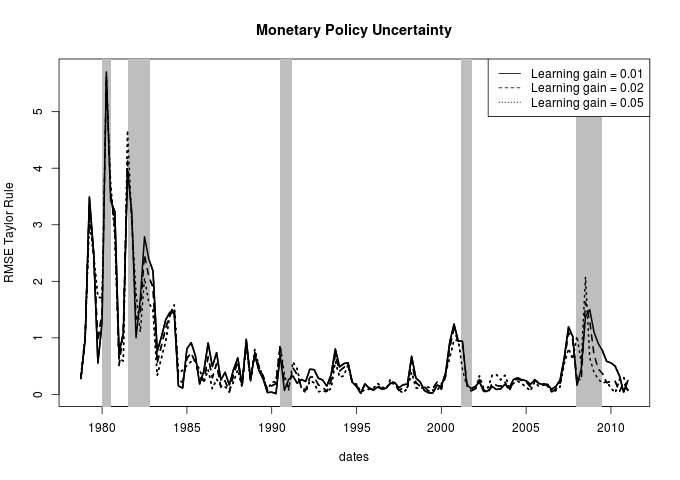
\includegraphics[scale=0.4]{mpu_ols.png} & 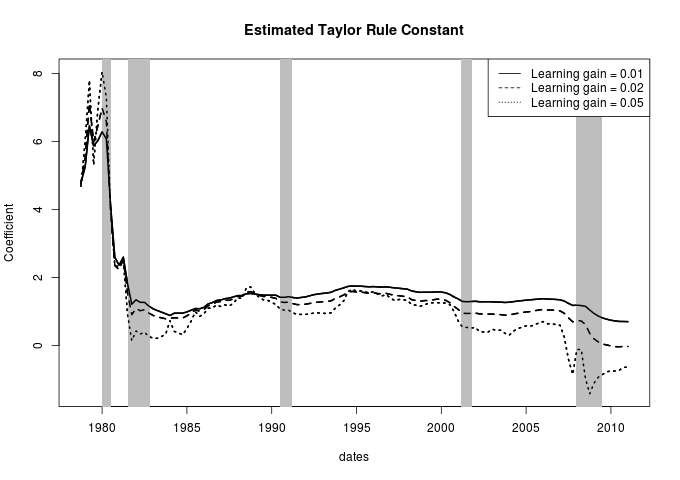
\includegraphics[scale=0.4]{coef_constant_ols.png} \\ [1pc]
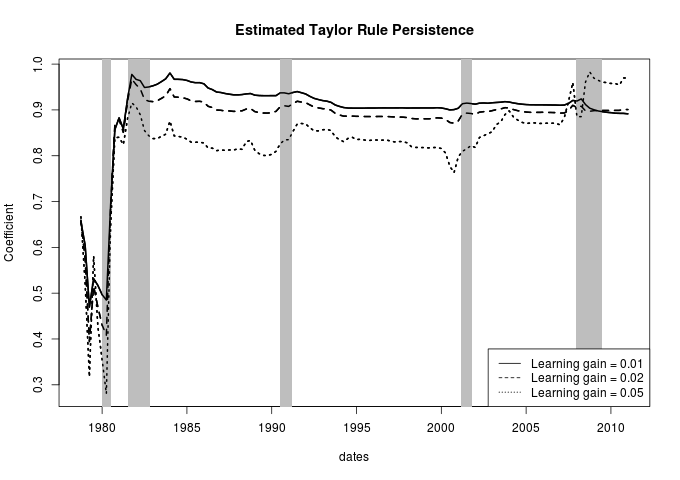
\includegraphics[scale=0.4]{coef_persistence_ols.png} & 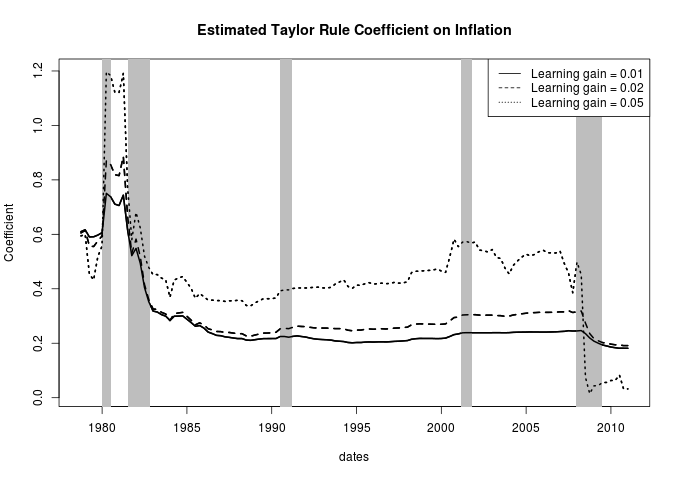
\includegraphics[scale=0.4]{coef_inflation_ols.png} \\
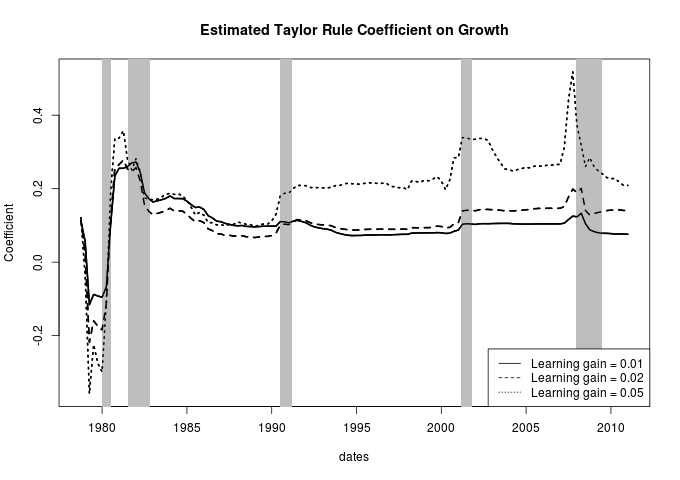
\includegraphics[scale=0.4]{coef_growth_ols.png} & 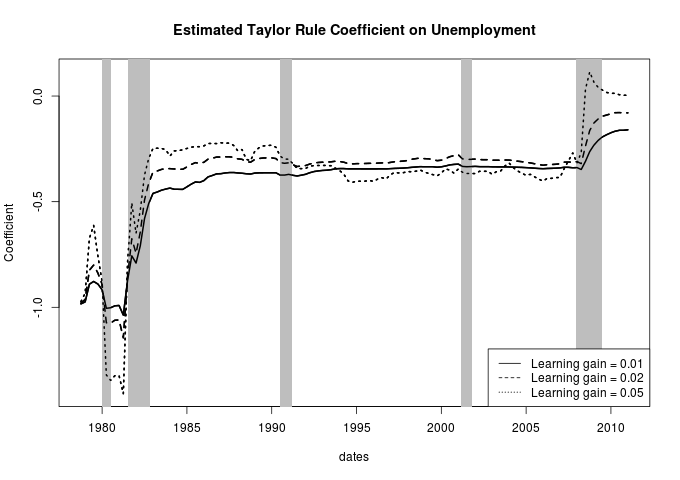
\includegraphics[scale=0.4]{coef_unemployment_ols.png} \\
\end{tabular}
\end{figure}

\begin{figure}\caption{Expectations With IV Learning: Uncertainty and Perceived Coefficients}\label{fg:coefs_iv}\vspace*{1pc}
\hspace*{-0.6in}\begin{tabular}{cc}
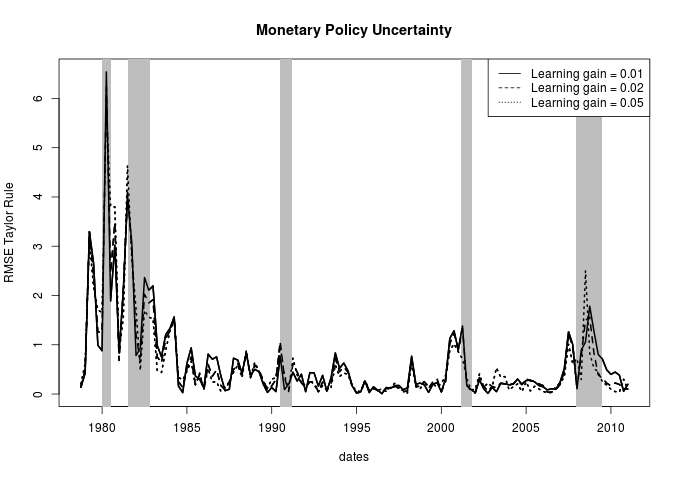
\includegraphics[scale=0.4]{mpu_iv.png} & 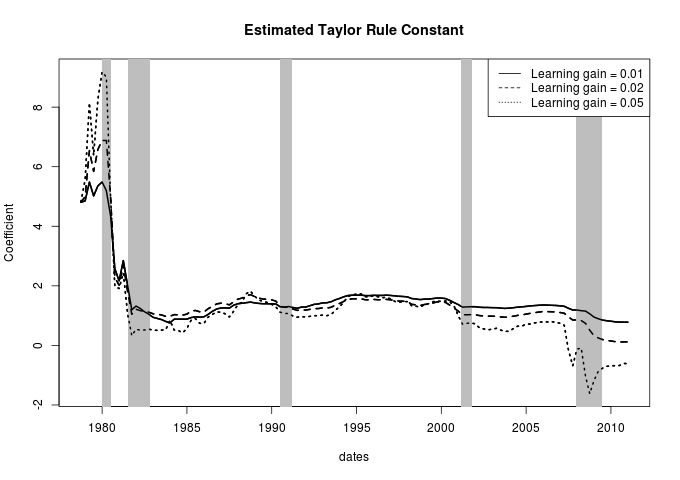
\includegraphics[scale=0.4]{coef_constant_iv.png} \\ [1pc]
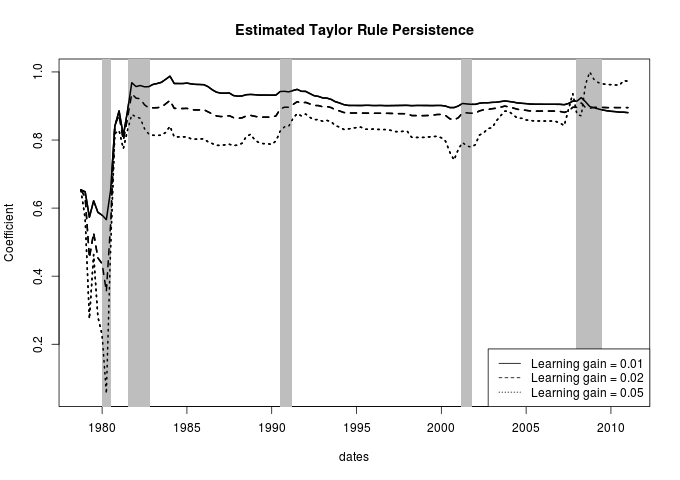
\includegraphics[scale=0.4]{coef_persistence_iv.png} & 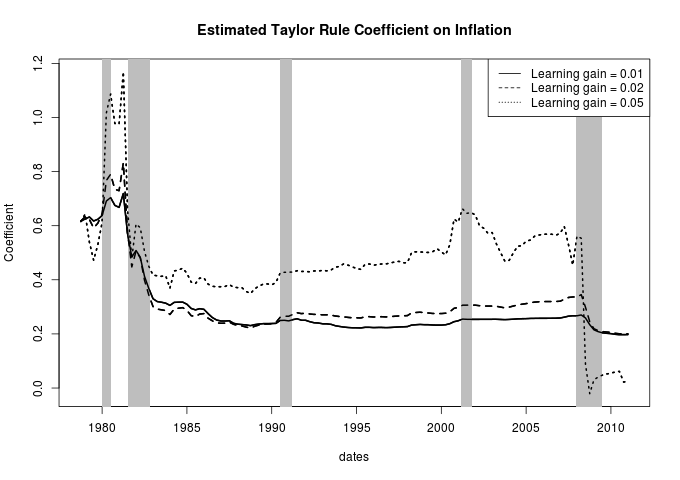
\includegraphics[scale=0.4]{coef_inflation_iv.png} \\
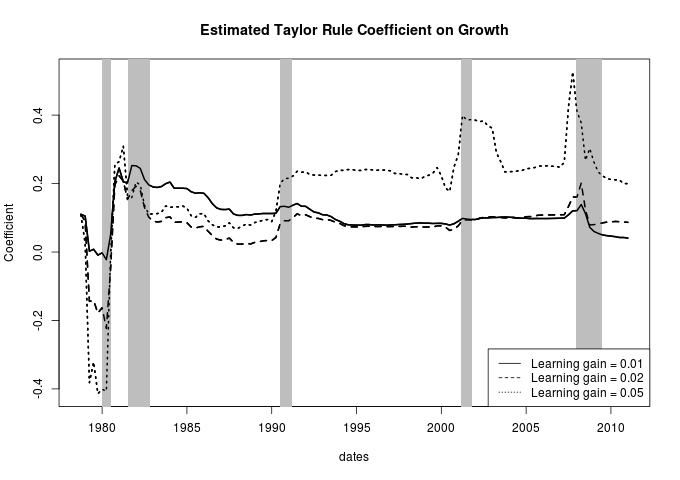
\includegraphics[scale=0.4]{coef_growth_iv.png} & 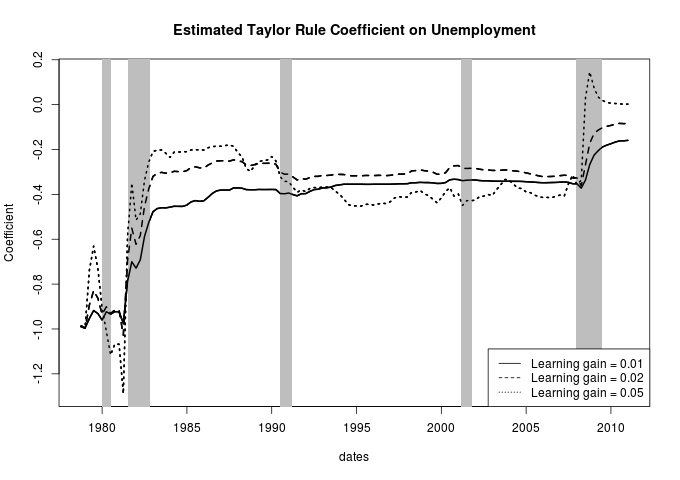
\includegraphics[scale=0.4]{coef_unemployment_iv.png} \\
\end{tabular}
\end{figure}

\end{document}


